\documentclass[a4paper,11pt]{extarticle}
\usepackage[a4paper]{geometry}
\geometry{verbose,tmargin=2cm,bmargin=2cm,lmargin=2cm,rmargin=2cm}

\usepackage{fontspec}
\defaultfontfeatures{Ligatures=TeX}
%\setmainfont{Linux Libertine O}
\setmainfont{FreeSerif}
%\setmonofont{Fira Mono}
\setmonofont{FreeMono}

\setlength{\parindent}{0cm}

\usepackage{float}
\usepackage{graphicx}

\usepackage{hyperref}
\usepackage{url}
\usepackage{xcolor}
\usepackage{amsmath}

\usepackage{minted}
%\newminted{julia}{breaklines,fontsize=\footnotesize}
\newminted{julia}{breaklines}

\begin{document}

\title{Electronic Structure Calculation using Plane Wave Basis Set}
\author{Fadjar Fathurrahman}
\date{}
\maketitle

\tableofcontents

\section{Introduction}

This document is part of package
{\tt ffr-ElectronicStructure.jl} using plane wave basis set.

\section{ {\tt PWGrid\_xx.jl} }

\verb|xx| stands for the version (or variant) of \verb|PWGrid|.


\subsection{ {\tt PWGrid\_01.jl} }

In this file, a type \verb|PWGrid| is defined:
\begin{juliacode}
type PWGrid
  Ns::Array{Int64}
  LatVecs::Array{Float64,2}
  RecVecs::Array{Float64,2}
  Npoints::Int
  Ω::Float64
  r::Array{Float64,2}
  G::Array{Float64,2}
  G2::Array{Float64}
end
\end{juliacode}

The fields of this type are:
\begin{itemize}

\item {\tt Ns} is an integer array which defines number of sampling points
in each lattice vectors.

\item {\tt LatVecs} is $3\times3$ matrix which defines lattice vectors of
unit cell in real space.

\item {\tt RecVecs} is $3\times3$ matrix which defines lattice vectors of
unit cell in reciprocal space. It is calculated according to \eqref{eq:recvecs}.

\item {\tt Npoints} Total number of sampling points
\item {\tt Ω} Unit cell volume in real space
\item {\tt r} Real space grid points
\item {\tt G} \textbf{G}-vectors
\item {\tt G2} Magnitude of \textbf{G}-vectors

\end{itemize}

Constructor for {\tt PWGrid} is defined as follow.
\begin{juliacode}
function PWGrid( Ns::Array{Int,1},LatVecs::Array{Float64,2} )
  Npoints = prod(Ns)
  RecVecs = 2*pi*inv(LatVecs')
  Ω = det(LatVecs)
  R,G,G2 = init_grids( Ns, LatVecs, RecVecs )
  return PWGrid( Ns, LatVecs, RecVecs, Npoints, Ω, R, G, G2 )
end
\end{juliacode}

The function \verb|init_grid()| is defined as follow. It takes
\verb|Ns|, \verb|LatVecs|, and \verb|RecVecs| as the arguments.
\begin{juliacode}
function init_grids( Ns, LatVecs, RecVecs )
\end{juliacode}

First, grid points in real space are initialized:
\begin{juliacode}
  Npoints = prod(Ns)
  r = Array(Float64,3,Npoints)
  ip = 0
  for k in 0:Ns[3]-1
  for j in 0:Ns[2]-1
  for i in 0:Ns[1]-1
    ip = ip + 1
    r[1,ip] = LatVecs[1,1]*i/Ns[1] + LatVecs[2,1]*j/Ns[2]
              + LatVecs[3,1]*k/Ns[3]
    r[2,ip] = LatVecs[1,2]*i/Ns[1] + LatVecs[2,2]*j/Ns[2]
              + LatVecs[3,2]*k/Ns[3]
    r[3,ip] = LatVecs[1,3]*i/Ns[1] + LatVecs[2,3]*j/Ns[2]
              + LatVecs[3,3]*k/Ns[3]
  end
  end
  end
\end{juliacode}

In the next step, grid points in reciprocal space, or \textbf{G}-vectors
and also their squared values are initialized
\begin{juliacode}
  G  = Array(Float64,3,Npoints)
  G2 = Array(Float64,Npoints)
  ip    = 0
  for k in 0:Ns[3]-1
  for j in 0:Ns[2]-1
  for i in 0:Ns[1]-1
    gi = mm_to_nn( i, Ns[1] )
    gj = mm_to_nn( j, Ns[2] )
    gk = mm_to_nn( k, Ns[3] )
    ip = ip + 1
    G[1,ip] = RecVecs[1,1]*gi + RecVecs[2,1]*gj + RecVecs[3,1]*gk
    G[2,ip] = RecVecs[1,2]*gi + RecVecs[2,2]*gj + RecVecs[3,2]*gk
    G[3,ip] = RecVecs[1,3]*gi + RecVecs[2,3]*gj + RecVecs[3,3]*gk
    G2[ip] = G[1,ip]^2 + G[2,ip]^2 + G[3,ip]^2
  end
  end
  end
\end{juliacode}

The function {\tt mm\_to\_nn} defines mapping from real space to Fourier space:
\begin{juliacode}
function mm_to_nn(mm::Int,S::Int)
  if mm > S/2
    return mm - S
  else
    return mm
  end
end
\end{juliacode}

Finally, the variables \verb|r|, \verb|G|, and \verb|G2| are returned.
\begin{juliacode}
  return r,G,G2
\end{juliacode}

We give an example of creating a {\tt PWGrid} object:
\begin{juliacode}
Ns = [40, 40, 40]
LatVecs = 10*diagm(ones(3))
pw = PWGrid( Ns, LatVecs )
\end{juliacode}


\section{Visualizing real-space grid points}

In the directory \verb|pwgrid_01|, we visualize grid points in real space
using Xcrysden program. Originally Xcrysden, is meant to visualize crystalline structure,
however, we also can use it to visualize grid points, taking periodic boundary
conditions into consideration.
This is useful to check whether grid points are generated correctly or not.

\begin{figure}
\centering
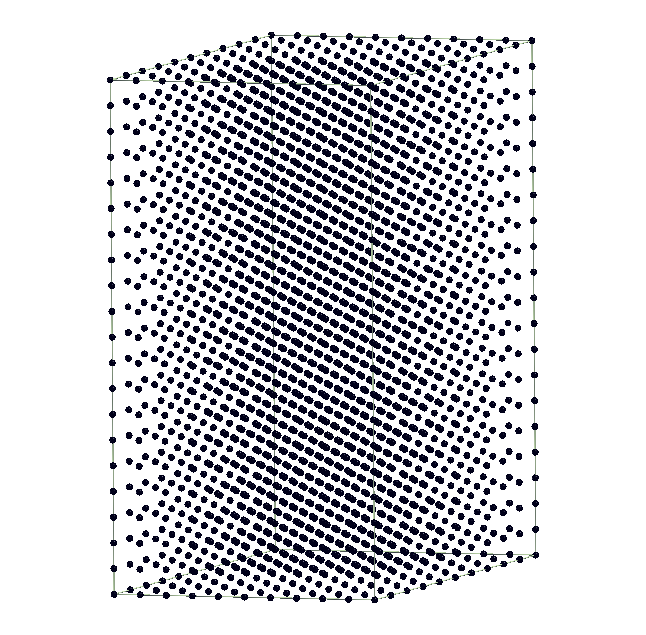
\includegraphics[scale=0.25]{images/R_grid_hexagonal.png}
\par
\end{figure}


\section{Solving Poisson equation}

Poisson equation is relatively easy to solve in periodic
boundary condition using Fourier method (FFT). This is different
from other discretization method, such as finite difference or Lagrange
function.

An example a program to solve Poisson equation is given in directory
{\tt poisson\_01}. In this program, a charge density is constructed
from difference between two Gaussian charge density. Total charge
(integrated charge density) is restricted to zero.
From this charge density, we calculate the electrostatic (Hartree) potential
by solving Poisson equation.

Function to generate vector \verb|dr|:
\begin{juliacode}
function gen_dr( r, center )
  Npoints = size(r)[2]
  dr = Array(Float64,Npoints)
  for ip=1:Npoints
    dx2 = ( r[1,ip] - center[1] )^2
    dy2 = ( r[2,ip] - center[2] )^2
    dz2 = ( r[3,ip] - center[3] )^2
    dr[ip] = sqrt( dx2 + dy2 + dz2 )
  end
  return dr
end
\end{juliacode}


Function to generate charge density:
\begin{juliacode}
function gen_rho( dr, σ1, σ2 )
  Npoints = size(dr)[1]
  rho = Array( Float64, Npoints )
  c1 = 2*σ1^2
  c2 = 2*σ2^2
  cc1 = sqrt(2*pi*σ1^2)^3
  cc2 = sqrt(2*pi*σ2^2)^3
  for ip=1:Npoints
    g1 = exp(-dr[ip]^2/c1)/cc1
    g2 = exp(-dr[ip]^2/c2)/cc2
    rho[ip] = g2 - g1
  end
  return rho
end
\end{juliacode}

Function to solve Poisson equation:
\begin{juliacode}
function solve_poisson( pw_grid::PWGrid, rho )
  Ω  = pw_grid.Ω
  G2 = pw_grid.G2
  Ns = pw_grid.Ns
  Npoints = pw_grid.Npoints
  ctmp = 4.0*pi*R_to_G( Ns, rho )
  for ip = 2:Npoints
    ctmp[ip] = ctmp[ip] / G2[ip]
  end
  ctmp[1] = 0.0
  phi = real( G_to_R( Ns, ctmp ) )
  return phi
end
\end{juliacode}


\section{Solving Schrodinger equation}

Using energy minimization:

Introduction to minimization

simple 2D minimization, using steepest-descent and conjugate gradient
method


Using iterative diagonalization: Davidson and LOBPCG

background information about iterative diagonalization
Eigenvalue problems


\chapter{Formulae}

Plane wave basis $b_{\alpha}(\mathbf{r})$:
\begin{equation}
b_{\alpha}(\mathbf{r}) = \frac{1}{\sqrt{\Omega}} e^{\mathbf{G}_{\alpha}\cdot\mathbf{r}}
\end{equation}

Lattice vectors of unit cell in reciprocal space:
\begin{equation}\label{eq:recvecs}
\mathbf{b} = 2\pi\left( a^{T} \right)^{-1}
\end{equation}

\textbf{G}-vectors:
\begin{equation}
\mathbf{G} = i \mathbf{b}_{1} + j \mathbf{b}_{2} + k \mathbf{b}_{3}
\end{equation}

Structure factor:
\begin{equation}
S_{I}(\mathbf{G}) = \sum_{\mathbf{G}} e^{ -\mathbf{G}\cdot\mathbf{X}_{I} }
\end{equation}



\end{document}
